\subsection{Menü-Struktur}\label{subsec:menu-struktur}

Im folgenden Abschnitt werden die einzelnen Menüs behandelt und erklärt. Vorab eine ausführliche Übersicht der Menü-Struktur:\\

\begin{figure}[H]
    \centering
    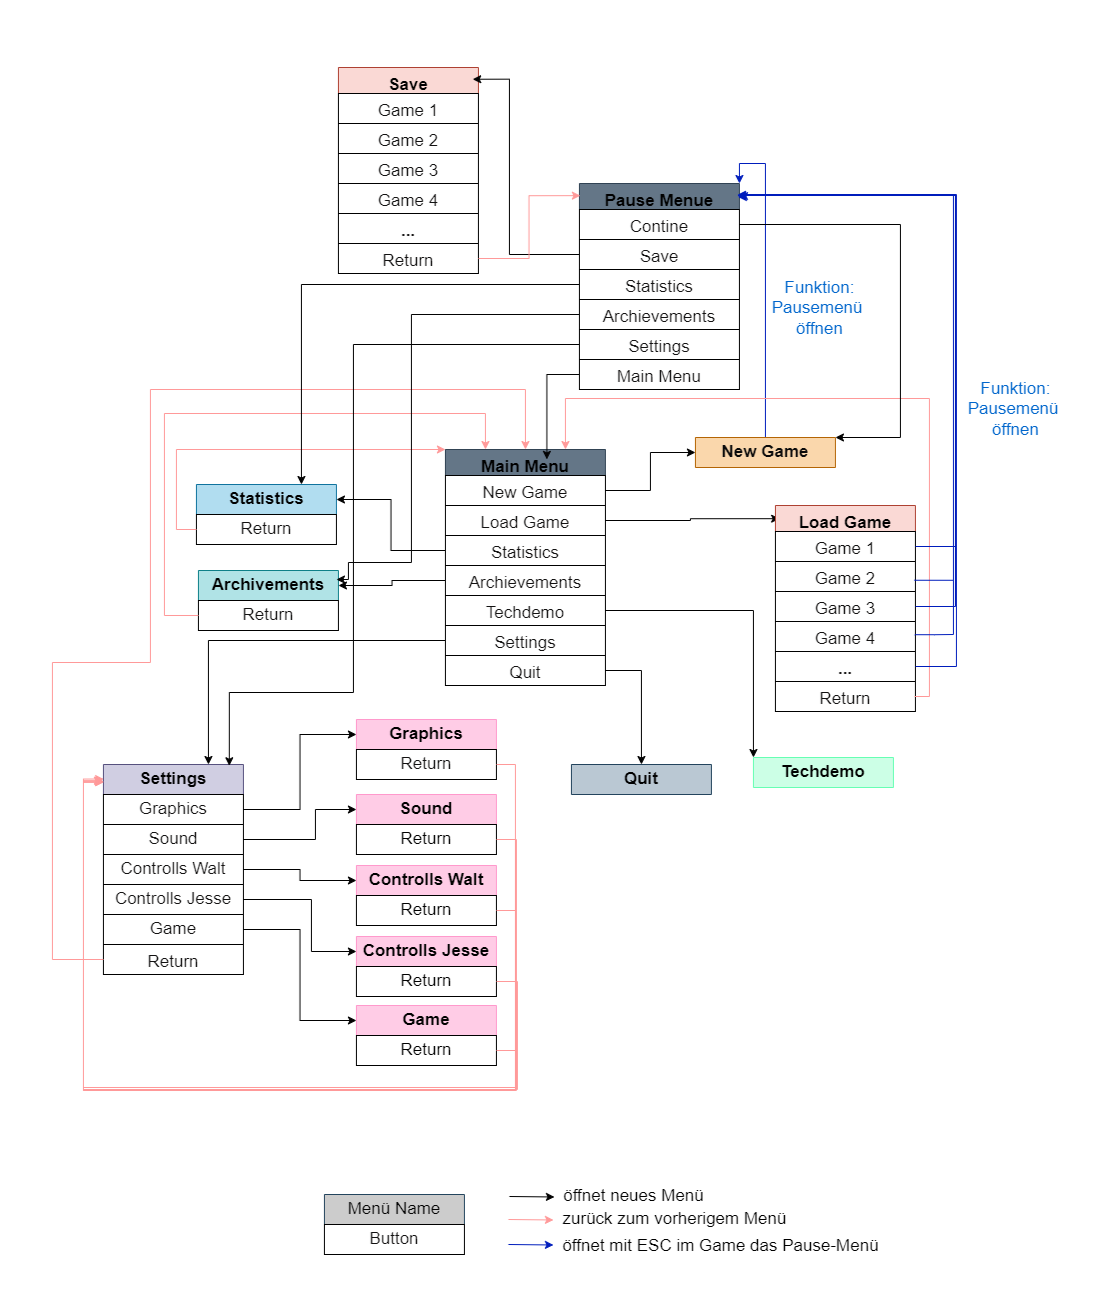
\includegraphics[width=1.0\textwidth]{figures/menuStructure}
    \caption{Menü-Struktur mit Legende}
    \label{fig:menuStructure}
\end{figure}

Nach dem Starten des Spiels wird das \textbf{Hauptmenü} mit folgenden Buttons angezeigt (Steuerung erfolgt über die Pfeiltasten oder die Maus):

\begin{itemize}
    \item \textbf{New Game:} startet ein neues Spiel mit einem neuen Speicherstand
    \item \textbf{Load Game:} Zeigt alle vorhanden Spielstände an und lädt den ausgewählten Spielstand
    \item \textbf{Statistics:} Zeigt eine Übersicht von allen vorhanden Statistiken an
    \item \textbf{Achievements:} Zeigt alle möglichen Achievements an, wie diese erreicht werden können und welche schon erreicht wurden
    \item \textbf{Settings:} Hier sind Einstellungen bezüglich des Sound, der Grafik und der Steuerung möglich: \newline
    - Controls Walt: Tastenbelegungen für Spieler1 personalisieren \newline
    - Controls Jesse: Tastenbelegungen für Spieler2 personalisieren \newline
    - Sound: Lautstärkeslider für Hintergrundmusik/Soundeffekte \newline
    - Grafik: Auswählen von Bildschirmauflösungspresets \newline
    - Game: Schwierigkeitsstufe: Leicht/Mittel/Schwierig
    \item \textbf{Quit:} Beendet das Spiel
\end{itemize}
Durch Drücken von [ESC] öffnet sich während des Spiels ein \textbf{Pausemenü}.

\begin{itemize}
    \item \textbf{Continue:} setzt das Spiel fort
    \item \textbf{Save:} Speichert den aktuellen Spielstand unter dem ausgewählten Slot
    \item  \textbf{Statistics:} Zeigt eine Übersicht von allen vorhanden Statistiken an
    \item  \textbf{Achievements:} Zeigt alle möglichen Achievements an, wie diese erreicht werden können und welche schon erreicht wurden
    \item \textbf{Settings:} Hier sind Einstellungen bezüglich des Sound, der Grafik und der Steuerung möglich: \newline
    - Controls Walt: Tastenbelegungen für Spieler1 personalisieren \newline
    - Controls Jesse: Tastenbelegungen für Spieler2 personalisieren \newline
    - Sound: Lautstärkeslider für Hintergrundmusik/Soundeffekte \newline
    - Grafik: Auswählen von Bildschirmauflösungspresets \newline
    - Game: Schwierigkeitsstufe: Leicht/Mittel/Schwierig
    \item \textbf{Main Menu:} öffnet das Hauptmenü
\end{itemize}
\newpage
